\begin{tikzpicture}
%    \def\lenreg{2};
%    \def\diam{3};
    \def\spy{2};
    \def\xdist{8cm};
    \def\ydist{-7cm};
%    \def\persp{20};
%    
%    \def\LX{1};
%    \def\LY{2};
%    \def\CoreX{1.5};
%    \def\CoreY{.9*\LY};
%    

	\def\L{2};
	\def\R{6};
	\def\HX{.25};
	\def\decalage{\R/2-\L/2};
    
%	Islam's idea
	\begin{scope}
%		\begin{tikzpicture}[scale=2/3]

%    \def\lenreg{2};
%    \def\diam{3};
    \def\spy{2};
    \def\xdist{8cm};
    \def\ydist{-7cm};
%    \def\persp{20};
%    
%    \def\LX{1};
%    \def\LY{2};
%    \def\CoreX{1.5};
%    \def\CoreY{.9*\LY};
%    

	\def\L{2.1};
	\def\R{5};
	\def\HX{.25};
	\def\decalage{\R/2-\L/2};
	
		\draw(6.5,\R/2) node{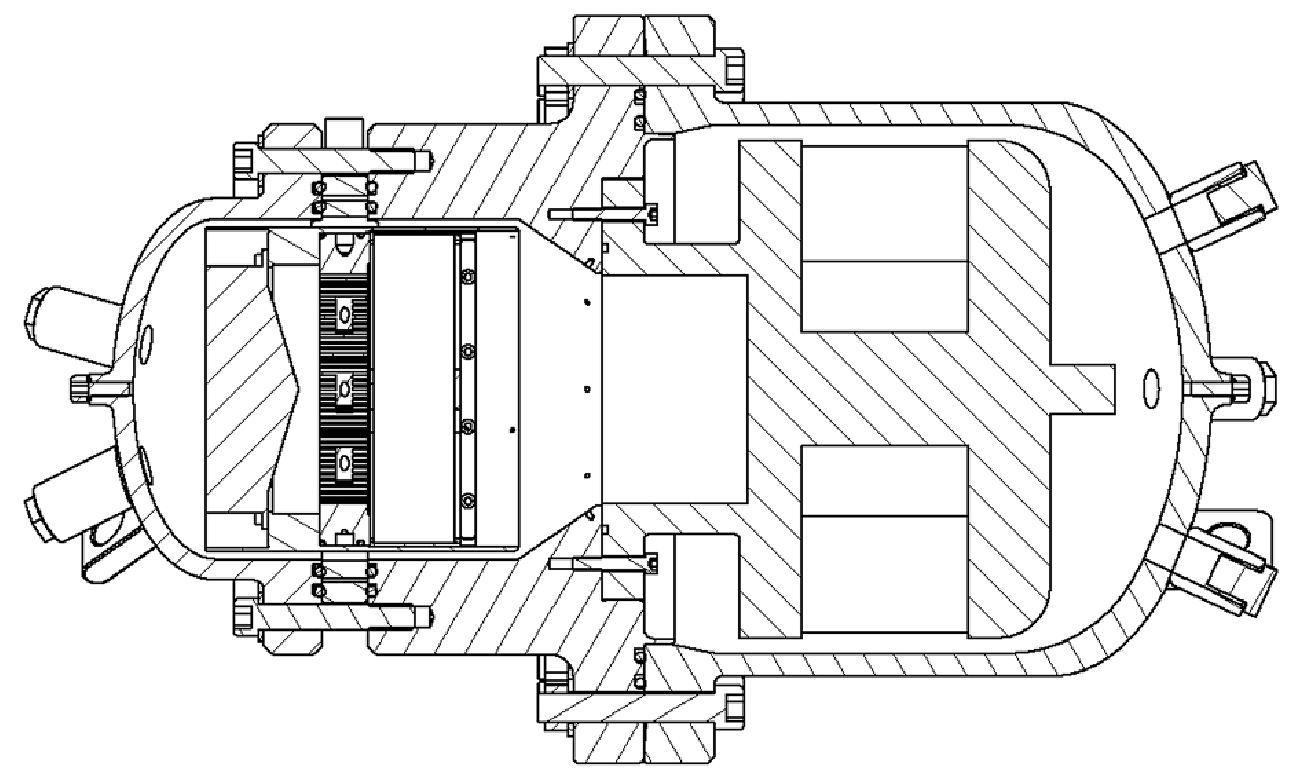
\includegraphics[width=.8\textwidth]{../fig/fig_OrientationCore/tex/TACOT.png}};
			
		\fill[right color=blue!25,left color=red!25, draw=black] (\decalage,0) rectangle ++(\L,\R);
		\draw[fill=red!25] (\decalage,0) rectangle ++(-\HX,\R);
		\draw[fill=blue!25] (\decalage+\L,0) rectangle ++(\HX,\R);

		\foreach \z [evaluate=\z] in {0,...,4}{
			\foreach \r [evaluate=\r as \num using int(\r+1 + 3*\z)] in {0,...,2}{
				\draw ({\decalage+.5+\L-\z*(1+\L)/4},{-(\R-.4)/2*\r+\R-.2}) node[minimum size=10pt,draw,circle,fill=white,opacity=.7,text opacity=1]{} node(n\z\r){\scriptsize \num};
}}

%		\draw (n01.east) node [right]{0 $\rightarrow$ \begin{tabular}{l}Source\\acoustique\\principale\end{tabular}};
		\draw ($(n01)+(1.5,0)$) node[minimum size=10pt,draw,circle,fill=white,opacity=.7,text opacity=1]{} node(RIX) {\scriptsize 0};% node[anchor=west]{\begin{tabular}{rl}
%		& Source\\
%		$\rightarrow$ & acoustique\\
%		& principale
%		\end{tabular}};
		\draw (n30.north west) node [above, fill=white, fill opacity=.7, text opacity=1]{Ambiant};
		\draw (n10.north east) node [above, fill=white, fill opacity=.7, text opacity=1]{Froid};
\end{tikzpicture}
		\fill[right color=blue!25,left color=red!25, draw=black] (\decalage,0) rectangle ++(\L,\R);
		\draw[fill=red!25] (\decalage,0) rectangle ++(-\HX,\R);
		\draw[fill=blue!25] (\decalage+\L,0) rectangle ++(\HX,\R);

		\foreach \z [evaluate=\z] in {0,...,4}{
			\foreach \r [evaluate=\r as \num using int(\r+1 + 3*\z)] in {0,...,2}{
				\draw ({\decalage+.5+\L-\z*(1+\L)/4},{-(\R-.4)/2*\r+\R-.2}) node(n\z\r){\num};
}}

		\draw (n01.east) node [right]{$\rightarrow$ \begin{tabular}{l}Source\\acoustique\\principale\end{tabular}};
		\draw (n30.north west) node [above]{AHX};
		\draw (n10.north east) node [above]{CHX};

		\draw (0,\R+\spy) node [anchor=west]{\textbf{(a)} \texttt{H1}};

	\end{scope}
	
	
	
	\begin{scope}[xshift=\xdist-1cm,yshift=2cm]
		\begin{scope}[xslant=1,yscale=.5]
%		\begin{tikzpicture}[scale=2/3]

%    \def\lenreg{2};
%    \def\diam{3};
    \def\spy{2};
    \def\xdist{8cm};
    \def\ydist{-7cm};
%    \def\persp{20};
%    
%    \def\LX{1};
%    \def\LY{2};
%    \def\CoreX{1.5};
%    \def\CoreY{.9*\LY};
%    

	\def\L{1};
	\def\R{5};
	\def\HX{.25};
	\def\decalage{\R/2-\L/2};
	
%	\draw[opacity=0] (\decalage,0) rectangle ++(-\HX,\R); %%% Pour l'alignement vertical
%\draw{[white](\L/2,0) -- ++(0,\R);
	
	\begin{scope}[yslant=-1]
		\begin{scope}[xslant=.71]%, rotate=90, xscale=1]
		\node at (\decalage-\HX,0) (NewO) {};
%		\draw[->, very thick] (NewO.center) -- ++(0,1.2*\R);
%		\draw[->, very thick] (NewO.center) -- ++(1.2*\R,0);
		
		\fill[shading=axis,right color=MatlabBlue,left color=MatlabOrange, shading angle=22.5, draw=black] (\decalage,0) rectangle ++(\L,\R*1.4);
		\draw[fill=MatlabOrange] (\decalage,0) rectangle ++(-\HX,\R*1.4);
		\draw[fill=MatlabBlue] (\decalage+\L,0) rectangle ++(\HX,\R*1.4);

		\foreach \z [evaluate=\z] in {0,...,4}{
			\foreach \r [evaluate=\r as \num using int(\r+1 + 3*\z)] in {0,...,2}{
				\draw ({\decalage+.5+\L-\z*(1+\L)/4},{-(\R*1.4-.4)/2*\r+\R*1.4-.2}) node[minimum size=10pt,draw,circle,fill=white,opacity=.7,text opacity=1]{} node(n\z\r){\scriptsize \num};
}}

%		\draw (n01.east) node [right]{$\rightarrow$ \begin{tabular}{l}Source\\acoustique\\principale\end{tabular}};
		\draw ($(n01)+(.75,0)$) node[minimum size=10pt,draw,circle,fill=white,opacity=.7,text opacity=1]{} node {\scriptsize 0};% node[anchor=west]{\begin{tabular}{rl}
%		& Src\\
%		$\rightarrow$ & ac\\
%		& princ
%		\end{tabular}};
%		\draw (n30.north west) node [above right, fill=white, fill opacity=0, text opacity=1]{\textcolor{MatlabOrange}{\textbf{Ambiant}}};
%		\draw (n10.north east) node [above right, fill=white, fill opacity=0, text opacity=1]{\textcolor{MatlabBlue}{\textbf{Froid}}};
		
	\end{scope}
	\end{scope}
	\begin{pgfonlayer}{background}
		\draw[->, very thick] (NewO.center) -- ++(22.5:1.2*\R) node [above] {$\mathbf e_{y,0}$};
		\draw[->, very thick] (NewO.center) -- ++(90:1.2*\R) node [left] {$\mathbf e_{z,0}$};
		\draw[->, very thick] (NewO.center) -- ++(-45:1.2*\R) node [right] {$\mathbf e_{x,0}$};
  	\end{pgfonlayer}
\end{tikzpicture}
		\fill[right color=blue!25,left color=red!25, draw=black] (\decalage,0) rectangle ++(\L,\R);
		\draw[fill=red!25] (\decalage,0) rectangle ++(-\HX,\R);
		\draw[fill=blue!25] (\decalage+\L,0) rectangle ++(\HX,\R);

		\foreach \z [evaluate=\z] in {0,...,4}{
			\foreach \r [evaluate=\r as \num using int(\r+1 + 3*\z)] in {0,...,2}{
				\draw ({\decalage+.5+\L-\z*(1+\L)/4},{-(\R-.4)/2*\r+\R-.2}) node(n\z\r){\num};
}}

		\draw (n01.east) node [right]{$\rightarrow$ \begin{tabular}{l}Source\\acoustique\\principale\end{tabular}};
		\draw (n30.north west) node [above]{AHX};
		\draw (n10.north east) node [above]{CHX};
		\end{scope}

		\draw (1cm,\R+\spy-2cm) node [anchor=west]{\textbf{(b)} \texttt{H2}};
	\end{scope}  
	
	
	  
	\begin{scope}[yshift=\ydist]
%		%\fill[top color=red!25, bottom color=blue!25, draw=black] (0,0) rectangle ++(\R,\L);
%\draw[fill=blue!25] (0,0) rectangle ++(\R,-\HX);
%\draw[fill=red!25] (0,\L) rectangle ++(\R,\HX);
%
%\foreach \z [evaluate=\z] in {0,...,4}{
%	\foreach \r [evaluate=\r as \num using int(\r+1 + 3*\z)] in {0,...,2}{
%		\draw ({-(\R-.4)/2*\r+\R-.2},{\z*(1+\L)/4-.5}) node(n\z\r){\num};
%}}
%
%\draw (n40.south east) node [right]{AHX};
%\draw (n00.north east) node[right]{CHX};
%\draw (n01.south) node [below]{\shortstack{ $\downarrow$ \\Source acoustique principale}};
%
%\draw (0,\L+2*\HX+\spy) node [anchor=west]{\textbf{(c)} \texttt{V1}};

\begin{tikzpicture}[scale=2/3]

%    \def\lenreg{2};
%    \def\diam{3};
    \def\spy{2};
    \def\xdist{8cm};
    \def\ydist{-7cm};
%    \def\persp{20};
%    
%    \def\LX{1};
%    \def\LY{2};
%    \def\CoreX{1.5};
%    \def\CoreY{.9*\LY};
%    

	\def\L{2};
	\def\R{5};
	\def\HX{.35};
	\def\decalage{\R/2-\L/2};
	
	\begin{scope}[yslant=tan(22.5)]	
		
		\node at (0,-\HX) (NewO) {};
	
		\fill[shading=axis,right color=MatlabBlue,left color=MatlabOrange, shading angle=22.5, draw=black] (0,0) rectangle ++(\R,\L);
		\draw[fill=MatlabBlue] (0,0) rectangle ++(\R,-\HX);
		\draw[fill=MatlabOrange] (0,\L) rectangle ++(\R,\HX);

		\foreach \z [evaluate=\z] in {0,...,4}{
			\foreach \r [evaluate=\r as \num using int(\r+1 + 3*\z)] in {0,...,2}{
				\draw ({-(\R-.4)/2*\r+\R-.2},{\z*(1+\L)/4-.5}) node[minimum size=10pt,draw,circle,fill=white,opacity=.7,text opacity=1]{} node(n\z\r){\scriptsize \num};
}}

%		\draw (n40.south east) node [right, fill=white, fill opacity=0, text opacity=1]{\textcolor{MatlabOrange}{\textbf{Ambiant}}};
%		\draw (n00.north east) node[right, fill=white, fill opacity=0, text opacity=1]{\textcolor{MatlabBlue}{\textbf{Froid}}};
		\draw ($(n01.south)+(0,-1.1)$) node[minimum size=10pt,draw,circle,fill=white,opacity=.7,text opacity=1]{} node (RIX){\scriptsize 0};% node[anchor=north]{\begin{tabular}{c}
%		$\downarrow$\\
%		Source acoustique principale
%		\end{tabular}};

	\end{scope}
	\begin{pgfonlayer}{background}
		\draw[->, very thick] (NewO.center) -- ++(22.5:1.2*\R) node [above] {$\mathbf e_{y,0}$};
		\draw[->, very thick] (NewO.center) -- ++(90:1.2*\R) node [left] {$\mathbf e_{z,0}$};
		\draw[->, very thick] (NewO.center) -- ++(-45:1.2*\R) node [right] {$\mathbf e_{x,0}$};
  	\end{pgfonlayer}		
\end{tikzpicture}		

		\fill[top color=red!25, bottom color=blue!25, draw=black] (0,0) rectangle ++(\R,\L);
		\draw[fill=blue!25] (0,0) rectangle ++(\R,-\HX);
		\draw[fill=red!25] (0,\L) rectangle ++(\R,\HX);

		\foreach \z [evaluate=\z] in {0,...,4}{
			\foreach \r [evaluate=\r as \num using int(\r+1 + 3*\z)] in {0,...,2}{
				\draw ({-(\R-.4)/2*\r+\R-.2},{\z*(1+\L)/4-.5}) node(n\z\r){\num};
}}

		\draw (n40.south east) node [right]{AHX};
		\draw (n00.north east) node[right]{CHX};
		\draw (n01.south) node [below]{\shortstack{ $\downarrow$ \\Source acoustique principale}};

		\draw (0,\L+2*\HX+\spy) node [anchor=west]{\textbf{(c)} \texttt{V1}};
	\end{scope} 
	
	
	
	   
	\begin{scope}[xshift=\xdist,yshift=\ydist]
%		%\fill[top color=blue!25, bottom color=red!25, draw=black] (0,0) rectangle ++(\R,\L);
%\draw[fill=red!25] (0,0) rectangle ++(\R,-\HX);
%\draw[fill=blue!25] (0,\L) rectangle ++(\R,\HX);
%
%\foreach \z [evaluate=\z] in {0,...,4}{
%	\foreach \r [evaluate=\r as \num using int(\r+1 + 3*\z)] in {0,...,2}{
%		\draw ({(\R-.4)/2*\r+.2},{-\z*(1+\L)/4+\L+.5}) node(n\z\r){\num};
%}}
%
%\draw (n01.north) node [above]{\shortstack{Source acoustique principale\\ $\uparrow$}};
%\draw (n42.north east) node [right]{AHX};
%\draw (n02.south east) node [right]{CHX};
%
%\draw (0,\L+2*\HX+\spy) node [anchor=west]{\textbf{(d)} \texttt{V2}};

\begin{tikzpicture}[scale=2/3]

%    \def\lenreg{2};
%    \def\diam{3};
    \def\spy{2};
    \def\xdist{8cm};
    \def\ydist{-7cm};
%    \def\persp{20};
%    
%    \def\LX{1};
%    \def\LY{2};
%    \def\CoreX{1.5};
%    \def\CoreY{.9*\LY};
%    

	\def\L{2.1};
	\def\R{5};
	\def\HX{.25};
	\def\decalage{\R/2-\L/2};

		\fill[top color=MatlabBlue, bottom color=MatlabOrange, draw=black] (0,0) rectangle ++(\R,\L);
		\draw[fill=MatlabOrange] (0,0) rectangle ++(\R,-\HX);
		\draw[fill=MatlabBlue] (0,\L) rectangle ++(\R,\HX);

		\foreach \z [evaluate=\z] in {0,...,4}{
			\foreach \r [evaluate=\r as \num using int(\r+1 + 3*\z)] in {0,...,2}{
				\draw ({(\R-.4)/2*\r+.2},{-\z*(1+\L)/4+\L+.5}) node[minimum size=10pt,draw,circle,fill=white,opacity=.7,text opacity=1]{} node(n\z\r){\scriptsize \num};
}}

		\draw ($(n01.north)+(0,1.1)$) node[minimum size=10pt,draw,circle,fill=white,opacity=.7,text opacity=1]{} node(RIX){\scriptsize 0};% node[anchor=south]{\begin{tabular}{c}
%		Source acoustique principale\\
%		$\uparrow$
%		\end{tabular}};
		\draw (n42.north east) node [right, fill=white, fill opacity=.7, text opacity=1]{\textcolor{MatlabOrange}{\textbf{Ambiant}}};
		\draw (n02.south east) node [right, fill=white, fill opacity=.7, text opacity=1]{\textcolor{MatlabBlue}{\textbf{Froid}}};
%		\draw (n41.south) node [below]{\textcolor{white}{\shortstack{Source acoustique principale\\ $\uparrow$}}};
		
\end{tikzpicture}	
		\fill[top color=blue!25, bottom color=red!25, draw=black] (0,0) rectangle ++(\R,\L);
		\draw[fill=red!25] (0,0) rectangle ++(\R,-\HX);
		\draw[fill=blue!25] (0,\L) rectangle ++(\R,\HX);

		\foreach \z [evaluate=\z] in {0,...,4}{
			\foreach \r [evaluate=\r as \num using int(\r+1 + 3*\z)] in {0,...,2}{
				\draw ({(\R-.4)/2*\r+.2},{-\z*(1+\L)/4+\L+.5}) node(n\z\r){\num};
}}

		\draw (n01.north) node [above]{\shortstack{Source acoustique principale\\ $\uparrow$}};
		\draw (n42.north east) node [right]{AHX};
		\draw (n02.south east) node [right]{CHX};

		\draw (0,\L+2*\HX+\spy) node [anchor=west]{\textbf{(d)} \texttt{V2}};	
	\end{scope}    
    
%	 Alternate version    
%    \draw[->] (5.5,-.5) -- ++(1,0);\draw(6,-1) node[]{Vertical 2};
%    \draw[->] (6.5,.5) -- ++(-1,0);\draw(6,1) node[]{Vertical 1};
%    \draw[->] (9,.5) -- ++(0,-1);\draw(9,1) node[]{Horizontal 1};
%    \draw (12,0) node[circle,draw]{.};\draw (12,1) node[]{Horizontal 2};
%    
%    
%    \draw[line width=.5mm] (-2.5*\LX,0) to[out=90,in=-180] (-\LX,\LY) -- ++(2*\LX,0) -- ++(.5*\LX,-2*\LY/3) -- ++(.2*\LX,0) -- ++(0,2*\LY/3);
\draw[line width=.5mm] (\LX,\LY) -- ++(\LX,0) to[out=0,in=90] (3.5*\LX,0);

\fill[left color=red,right color=blue] ({-\LX+.4*\CoreX},0) rectangle ({-\LX+.9*\CoreX},\CoreY);
\draw[line width=.5mm] (-\LX,\CoreY) -- ++(\CoreX,0);
\draw[fill=PythonBlue] (-.9*\LX,0) -- ++(0,\CoreY) to[out=-80,in=90] (-.7*\LX,0);
\draw ({-\LX+.4*\CoreX},0) -- ++(0,\CoreY);
\draw ({-\LX+.9*\CoreX},0) -- ++(0,\CoreY);

\draw[fill=PythonBlue] (1.6*\LX,0) |- ++(.3*\LX,.9*\LY/3) |- ++(\LX,.2*\LY) arc (90:0:.05) -- ++(0,-.5*\LY);
%    \begin{scope}[yscale=-1]
%        \draw[line width=.5mm] (-2.5*\LX,0) to[out=90,in=-180] (-\LX,\LY) -- ++(2*\LX,0) -- ++(.5*\LX,-2*\LY/3) -- ++(.2*\LX,0) -- ++(0,2*\LY/3);
\draw[line width=.5mm] (\LX,\LY) -- ++(\LX,0) to[out=0,in=90] (3.5*\LX,0);

\fill[left color=red,right color=blue] ({-\LX+.4*\CoreX},0) rectangle ({-\LX+.9*\CoreX},\CoreY);
\draw[line width=.5mm] (-\LX,\CoreY) -- ++(\CoreX,0);
\draw[fill=PythonBlue] (-.9*\LX,0) -- ++(0,\CoreY) to[out=-80,in=90] (-.7*\LX,0);
\draw ({-\LX+.4*\CoreX},0) -- ++(0,\CoreY);
\draw ({-\LX+.9*\CoreX},0) -- ++(0,\CoreY);

\draw[fill=PythonBlue] (1.6*\LX,0) |- ++(.3*\LX,.9*\LY/3) |- ++(\LX,.2*\LY) arc (90:0:.05) -- ++(0,-.5*\LY);
%    \end{scope}
    
    % Old version
    % %%%%%%%%%%%%%%%%%%%% V1
    % \fill[bottom color=PythonBlue, top color=PythonRed,draw=black] (-\xdist,{\ydist+\lenreg}) -- ++(0,{-\lenreg}) arc (0:-180:{\diam} and {\diam/\persp}) -- ++(0,{\lenreg}) arc (-180:0:{\diam} and {\diam/\persp}) --cycle;
    
    % \draw[fill=PythonRed] ({-\xdist-\diam},\ydist+\lenreg) ellipse ({\diam} and {\diam/\persp});
    
    % \draw ({-\xdist-\diam},\ydist-\spy) node []{\textbf{(a)} V1};
    
    
    % %%%%%%%%%%%%%%%%%%%% V2
    % \fill[bottom color=PythonRed, top color=PythonBlue,draw=black] (\xdist,{\ydist+\lenreg}) -- ++(0,{-\lenreg}) arc (-180:0:{\diam} and {\diam/\persp}) -- ++(0,{\lenreg}) arc (0:-180:{\diam} and {\diam/\persp}) --cycle;
    
    % \draw[fill=PythonBlue] ({\xdist+\diam},\ydist+\lenreg) ellipse ({\diam} and {\diam/\persp});
    
    % \draw ({\xdist+\diam},\ydist-\spy) node []{\textbf{(b)} V2};
    
    
    % %%%%%%%%%%%%%%%%%%%% H1
    % \draw ({-\xdist-\diam},-\ydist) circle (\diam);
    % \draw[dashed,very thick] ({-\xdist-\diam},{-\ydist+\diam}) -- ++(0,-2*\diam);
    
    % \draw ({-\xdist-\diam},-\ydist-\diam-\spy) node []{\textbf{(c)} H1};
    
    
    % %%%%%%%%%%%%%%%%%%%% H2
    % \draw ({\xdist+\diam},-\ydist) circle (\diam);
    % \draw[dashed,very thick] ({\xdist},{-\ydist}) -- ++(2*\diam,0);
    
    % \draw ({\xdist+\diam},-\ydist-\diam-\spy) node []{\textbf{(d)} H2};
\end{tikzpicture}